

\chapter{Methodisches Vorgehen einer EEG-Validierungsstudie}




\section{Beschreibung der Messapparatur}
Katharina \newline

Die Geräte, die miteinander verglichen werden, nutzen beide nicht-invasive Elektroden und schicken die gemessenen Daten digital an einen Rechner. Die Geräte werden zur Forschung genutzt. Die gleiche Einteilung der genutzten Geräte ermöglicht eine bessere Vergleichbarkeit.\newline

Das EEG, das als Vergleich dient, wird mit einem BioSemi ActiveTwo-System aufgezeichnet. 32 Elektroden werden an einer Kappe mit festen Positionen angebracht. Die Pin-Typ-Elektroden sind \Gls{silber-silberchlorid-elektrode}, trocken, langzeitstabil und wie in Abbildung \ref{pinelectroden} aufgebaut. Sie sind in dem erweiterten 10-20-System angeordnet. \newline

\begin{figure}
	\centering
	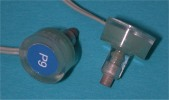
\includegraphics[width=0.325\textwidth]{bilder/Pin-Elektroden.jpg}
    \quelle{\cite{biosemi_active_electrodes}}
   \caption{Die Elektroden, die in einem BioSemi ActiveTwo-System genutzt werden}
   \label{pinelectroden}
\end{figure}

Anstatt Ground- und Referenzelektroden wird ein \acrshort{cms} / \acrshort{drl}-Kreis genutzt. Dabei wird die CMS-Elektrode in der Mitte aller messenden Elektroden angebracht und die DRL-Elektrode entfernt vom Kopf, zum Beispiel am Bein oder Arm.\footnote{ Vgl. \cite{biosemi_systems}} \newline
Ein Teil der Messungen (siehe 3.3.1) findet in einer speziellen, für EEGs ausgelegten Kabine (4400 A-CT-Special) von Industrial Acoustics statt.\footnote{ Vgl. \cite{iac_eeg_kabine}} Sie ist schwach beleuchtet, elektrisch isoliert und schallgedämpft, um die Aufnahme äußerer, nichtmenschlicher elektrischer Signale zu minimieren. Der Proband legt seinen Kopf in eine Kinnstütze und hat einen konstanten Abstand von 90 cm zum Monitor, auf dem die Experimente präsentiert werden.\newline

Das portable EEG-Gerät, das validiert werden soll, ist das Ultracortex Mark IV von OpenBCI. Es besteht aus einer 3D-gedruckten Halterung, welche auf das 10-20-System ausgelegt ist, in der 16 Silber-Silberchlorid-Elektroden eingesetzt werden. 14 davon sind trocken und mit spitzen Zacken versehen, um durch das Haar zu dringen. Die restlichen zwei sind ebenfalls trocken, haben aber keine Zacken, um auf die Haut aufgelegt zu werden und nicht zu verletzen. Sie werden an der Stirn angebracht. Alle Elektroden haben eine Lebensdauer von etwa zehn Nutzungen ohne Pflege, da die Beschichtung abgenutzt wird und sie schlechter leitet. Um eine korrekte Messung zu garantieren, müssen sie regelmäßig ausgetauscht werden.\footnote{ Vgl. \cite{openbci_dry_electrodes}}\newline 
Zusätzlich zu den messenden Elektroden enthält das System zwei Ohrclips, die als Referenzelektroden fungieren und keine Gehirnaktivität messen.\footnote{ Vgl. \cite{openbci_ultracortex_shop}} Verbunden werden die Elektroden mit Kabeln, die zu einer Platine führen, die die gesammelten Daten über Bluetooth an ein verbundenes Gerät schickt. Der Aufbau ist in Abbildung \ref{headset} zu sehen. \newline

\begin{figure}
	\centering
	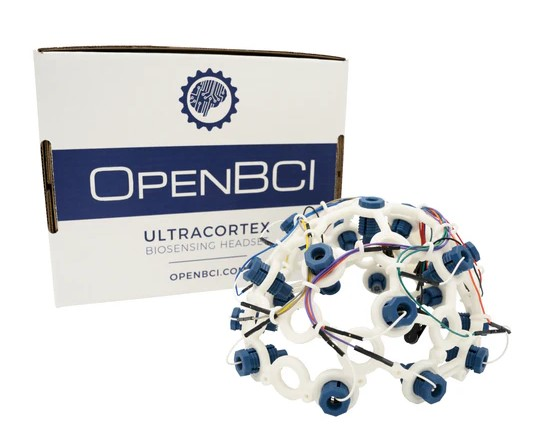
\includegraphics[width=0.325\textwidth]{bilder/Ultracortex_Headset.jpg}
   \quelle{\cite{openbci_ultracortex_shop}}
    \caption{Das Ultracortex Mark IV Headset}
    \label{headset}
\end{figure}

\section{Beschreibung der Stichprobe} 
Lorenz \newline

Es nehmen 15--20 Probanden an der Studie von April bis Juni 2026 teil. Sie sind zwischen 16 und 18 Jahren alt und besuchen das Carl-Zeiss-Gymnasium in der elften Klasse. Bevor ein EEG aufgenommen wird, unterschreiben die Teilnehmer eine schriftliche Einverständniserklärung, füllen einen Händigkeitsfragebogen aus und geben demografische Daten, wie Alter und Geschlecht, an. Ein genehmigter Ethik-Antrag unterstützt das Aufnehmen von Daten von Minderjährigen. Die Versuchspersonen absolvieren EEG-Messungen unter drei verschiedenen Bedingungen, die jeweils etwa zehn Minuten dauern. Dabei werden zwei etablierte Formen der Hirnaktivität erfasst: \Romannum{1}. visuelles ERP (auch P1 genannt) und \Romannum{2}. die Alpha-Power.

\section{Experimentalaufbau für die Messung} 
Lorenz \newline
\subsection{Versuchsbedingungen}
Lorenz \newline
Unsere Datenerhebung gliedert sich in drei Versuchsbedingungen, die von den Probanden durchlaufen werden. Die Versuchsbedingungen sind dabei folgendermaßen aufgebaut: \\
\begin{tabularx}{\textwidth}{@{}lX@{}}
-- \textbf{Versuchsbedingung 1:} & Die Messung findet mit dem OpenBCI-Gerät und ohne Kinnstütze statt, zudem ist die spezielle Kabine geöffnet, um möglichst alltagsnahe Situationen zu simulieren.  \\
-- \textbf{Versuchsbedingung 2:} & Die Messung findet mit dem OpenBCI-Gerät statt, nun mit einer Kinnstütze, und die Tür der Kabine ist geschlossen. \\
-- \textbf{Versuchsbedingung 3:} & Die Messung findet mit dem stationären EEG-System statt, unter idealen Bedingungen, d.h. die Kabine ist geschlossen und der Proband befindet sich in einer Kinnstütze. \\
\end{tabularx}
Dabei wurde zudem darauf geachtet, dass die Rahmenbedingungen konstant sind. Das beinhaltet gleichbleibende Beleuchtungsstärke und einen konstanten Geräuschpegel.

%\noindent Wenn Bedingung B erfüllt ist, wird ...
%\noindent Wenn Bedingung C erfüllt ist, wird ...

\subsection{Messung mit stationärem EEG-System}
Zur Erhebung der EEG-Daten werden den Probanden verschiedene Spielkarten auf einem Bildschirm aus einem Pokerdeck gezeigt. Jede Karte erscheint zweimal, einmal in großer Darstellung und einmal deutlich verkleinert mit reduziertem Kontrast. Mit dem Erscheinen jeder Karte wird ein zeitlicher Marker in den EEG-Rohdaten gesetzt. Dies ist ein wichtiger Bestandteil der Messung und hilft uns dabei, während der Auswertung genau zu lokalisieren, wann das Bild gezeigt wurde und wie die entsprechende Reaktion darauf ist. Denn nach der Präsentation eines Bildes tritt innerhalb der nächsten Millisekunden ein visuelles ERP (\Romannum{1}) auf. Dies ist gekennzeichnet durch einen charakteristischen Verlauf. Dabei ist eine bestimmte Komponente in diesem Verlauf für unsere Auswertungsmethode entscheidend: die sogenannte P1. Diese spiegelt die Verarbeitung des visuellen Reizes wider und reagiert sensibel auf Unterschiede in Größe und Kontrast der dargebotenen Reize. Entsprechend wird erwartet, dass sich die P1-Antwort zwischen den beiden Darstellungsbedingungen deutlich unterscheidet.
Ein einzelner Durchgang beginnt mit der Präsentation eines Fixationskreuzes für 500 ms, gefolgt von der Anzeige einer Spielkarte für 750 ms. Anschließend erscheint für 2000 ms ein schwarzer Bildschirm. Um die Aufmerksamkeit der Teilnehmenden sicherzustellen, sollen sie bei jedem gezeigten König die Leertaste drücken. Insgesamt werden 104 Karten präsentiert (52 Karten eines Pokerdecks in zweifacher Wiederholung), was eine Dauer von etwa fünf Minuten ergibt.
Um die Alpha-Power messen zu können (\Romannum{2}), wird das EEG einmal mit geschlossenen Augen aufgezeichnet und anschließend mit geöffneten. Zwischen diesen Bedingungen sollte ein großer Unterschied in der Alpha-Power zu sehen sein. Denn bei geschlossenen Augen ist die Alpha-Power größer als bei geöffneten. Diese Messung, inklusive Instruktion, dauert 3 Minuten.




    \subsection{Messung mit portablem EEG-System}

Zur Erhebung der EEG-Daten durchlaufen die Probanden den bereits in Abschnitt 3.3.2 beschriebenen Untersuchungsablauf, wobei die gleichen Aufgaben bearbeitet werden und sich lediglich die eingesetzten Messinstrumente unterscheiden. Zuerst durchläuft der Proband \textbf{Versuchsbedingung 1}, diese Daten werden aufgezeichnet und gespeichert. Im Anschluss durchläuft der Proband \textbf{Versuchsbedingung 2}.

  

    \subsection{Zeitlicher Ablauf des Experiments} 
    Lorenz \newline

Der geplante Ablauf sieht dabei folgendermaßen aus: 

    \begin{itemize}
\item Ankommen der ProbandInnen + Unterschreiben einer Einverständniserklärung (ca. 5 min.)
\item Erhebung der demografischen Daten (ca. 10 min)
\item Anlegen und Prüfen des portablen EEG-Systems (OpenBCI) (ca. 10 min)
\begin{itemize}
\item \textbf{Versuchsbedingung 1} (ca. 10 min)
\item \textbf{Versuchsbedingung 2} (ca. 10 min)
\end{itemize}
\item Abnehmen des portablen EEG-Systems und Anlegen des stationären EEG-Systems mit 32 Elektroden (ca. 25 min)
\begin{itemize}
\item \textbf{Versuchsbedingung 3}, Daten (\Romannum{1}. und \Romannum{2}.) (ca. 10 min)
\end{itemize}
\item Abnehmen des stationären Systems (ca. 5 min)
\item Haare waschen (ca. 10 min)
\item Belohnung, Auswertung, aufkommende Fragen besprechen, Verabschiedung der ProbandInnen (ca. 10 min) 

\end{itemize}

Für die Datenerhebung mit unseren ProbandInnen planen wir eine Gesamtdauer von etwa 110 Minuten pro Person ein. Diese Zeit umfasst sowohl die eigentliche EEG-Messung als auch die Vor- und Nachbereitung im Labor.
\section{Auswertungsmethodik}
Alisa \newline

Die im vorangegangenen Abschnitt beschriebenen Rohdaten werden für beide Zielgrößen -- die P1-Komponente und die Alpha-Power -- zunächst gemeinsam vorverarbeitet und anschließend in zwei getrennten Auswertungssträngen analysiert. Der grundsätzliche Ablauf ist in der Abbildung ..... dargestellt.

% ANMERKUNG: Platzhalter "....." für die Abbildungsreferenz war im Original
% noch nicht ausgefüllt - unverändert gelassen, da inhaltlich nicht meine
% Entscheidung.

\subsection{Vorverarbeitung der Rohdaten}

Vor der eigentlichen Analyse werden die Rohdaten für jede Versuchsperson bandpassgefiltert, das bedeutet, dass nur Frequenzen in einem bestimmten Frequenzbereich erhalten bleiben und alles darüber und darunter entfernt wird. Dadurch werden sowohl langsame Schwankungen (Drifts) als auch sehr hochfrequentes Rauschen entfernt. Drifts sind langsame Veränderungen der Spannungen, die durch Schwitzen oder schlechten Elektrodenkontakt entstehen. Hochfrequente Störungen, die zum Beispiel durch Muskelanspannung oder die Elektronik entstehen, werden ebenfalls entfernt. Am Ende bleibt nur der Frequenzbereich übrig, in dem die interessierende Hirnaktivität tatsächlich liegt. Anschließend wird mit einem \gls{notch}-Filter das durch das Wechselstromnetz verursachte 50-Hz-Netzbrummen (Rauschen) entfernt. Danach erfolgt eine Re-Referenzierung auf die Durchschnittsreferenz. Das bedeutet, dass die Spannungen aller Elektroden gemittelt werden und diese Mittelspannung von allen Elektroden abgezogen wird. Dadurch werden Spannungsunterschiede zwischen den Elektroden reduziert, um die Signalqualität zu verbessern. Da sich die Anforderungen der beiden Zielgrößen, der P1-Komponente und der Alpha-Power, unterscheiden, werden die Daten anschließend in zwei getrennten Auswertungssträngen weiterverarbeitet. Ereigniskorrelierte Potenziale benötigen eine feinere zeitliche Auflösung im niederfrequenten Bereich, während die Alpha-Power-Analyse ein breiteres Spektrum im mittleren Frequenzbereich abdeckt. Deshalb bekommt jeder der beiden Auswertungszweige (ERPs und Alpha-Power) seine eigenen, auf die jeweilige Zielgröße abgestimmten Filtergrenzen, statt beide mit denselben Grenzen zu behandeln. Elektroden, die während der Messung als defekt oder stark verrauscht auffielen, werden markiert und gehen im weiteren Verlauf nicht wie normale Elektroden unverändert in die weiteren Berechnungen ein, sodass diese nicht verfälscht werden. Dagegen werden sie repariert, also aus Nachbarelektroden rechnerisch ersetzt (Interpolation), und anschließend in die weiteren Berechnungen einbezogen. Die Interpolation erfolgt über die 3D-Positionen der Elektroden, die in der Kappe festgelegt sind. Die Positionen werden genutzt, um die Spannungen der Nachbarelektroden zu bewerten und daraus die Spannung der defekten Elektrode zu berechnen. 

% ANMERKUNG: Der Satz zu den defekten Elektroden ("...werden markiert und
% im weiterern Verlauf nicht wie normalen Elektroden, in die weiteren
% Berechnungen eingehen und diese verfälschen.") war im Original
% grammatisch nicht schlüssig (die Verneinung "nicht" bezog sich unklar
% auf einen oder beide der folgenden Verben). Ich habe die Satzstruktur so
% wenig wie möglich angepasst, um den aus dem Kontext eindeutigen Sinn
% (defekte Elektroden fließen NICHT unverändert in die Berechnung ein und
% verfälschen sie folglich auch nicht) grammatisch korrekt herzustellen -
% bitte gegenlesen, ob das genau eure gemeinte Aussage trifft.

\subsection{Auswertung der ereigniskorrelierten Potenziale (P1)}

Da einzelne Aktionspotenziale und selbst einzelne ereigniskorrelierte Antworten im fortlaufenden EEG nicht direkt erkennbar sind, sondern von deutlich größeren Hintergrundschwankungen überlagert werden (vgl. Abschnitt 2.4.6), lässt sich die P1-Komponente nicht aus einer einzelnen Reizsetzung ablesen. Sie muss stattdessen aus vielen gleichartigen Reizwiederholungen herausgemittelt werden. Die Auswertung der P1-Komponente gliedert sich deshalb in mehrere aufeinanderfolgende Schritte, die zunächst pro Versuchsperson und erst am Ende über die gesamte Stichprobe hinweg durchgeführt werden.

% ANMERKUNG: "Abschnitt 2.4.6" (und weiter unten "Abschnitt 2.4.7")
% verweisen auf die Gliederung von Kapitel 2. Da sich diese Gliederung im
% Lauf der Bearbeitung verschoben haben könnte, bitte prüfen, ob die
% Nummern noch stimmen - ich habe hier bewusst keine Zahl geraten/geändert.

\textbf{Epochierung:} Zunächst wird die fortlaufende Aufzeichnung jeder Versuchsperson um jeden einzelnen Bild Reiz herum in kurze Ausschnitte, sogenannte Epochen, zerschnitten. Jede Epoche beginnt kurz vor dem jeweiligen Reizbeginn und reicht bis knapp eine Sekunde danach, sodass sowohl ein Referenzzeitraum vor dem Reiz als auch der gesamte relevante Antwortverlauf danach erfasst wird. Die beiden Darbietungsbedingungen groß/normalkonstratiert und klein/kontrastreduziert (vgl. Abschnitt 3.3.1)  werden dabei von Anfang an getrennt gehalten, da sie später getrennt gemittelt und miteinander verglichen werden sollen. In diesem Schritt findet noch keine Basislinienkorrektur statt; sie wird bewusst erst nach der Artefaktbereinigung durchgeführt (siehe unten).


\textbf{Manuelle Epochierung:} Nicht jede Epoche eignet sich für die weitere Auswertung: Bewegt sich eine Versuchsperson, verspannt sie die Kiefer- oder Nackenmuskulatur oder löst sich kurzzeitig eine Elektrode, entstehen große, kurzzeitige Spannungsausschläge, die das später berechnete Mittel verzerren würden. Anstatt solche Epochen anhand eines einzelnen, fest gewählten Amplitudengrenzwerts automatisch zu verwerfen, werden alle Epochen visuell durchgesehen und einzeln beurteilt. Diese Vorgehensweise wurde gewählt, da ein fester Schwellenwert bei realen, unterschiedlich stark verrauschten Aufzeichnungen entweder zu viele unauffällige Epochen mitverwirft oder zu viele gestörte Epochen durchlässt. Die visuelle Beurteilung erlaubt es dagegen, für jede Epoche einzeln zwischen echten Artefakten und normaler Signalvariabilität zu unterscheiden. Die Epochen, die als gestört erkannt werden, werden aus der weiteren Analyse ausgeschlossen. 


\textbf{Artefaktkorrektur mittels ICA:} Im nächsten Schritt wird eine Unabhängigkeitskomponentenanalyse (Independent Component Analysis, ICA) auf die verbleibenden Epochen angewendet. Ziel ist es, das gemessene Gesamtsignal, das an jeder Elektrode immer eine Überlagerung mehrerer gleichzeitig aktiver Quellen enthält, rechnerisch in eine vorgegebene Anzahl statistisch unabhängiger Komponenten zu zerlegen. Einige Störquellen zeigen dabei typische räumliche und zeitliche Muster. So erzeugen Lidschläge starke Ausschläge, die vor allem an der Stirn konzentriert sind. Horizontale Augenbewegungen zeigen sich als entgegengesetzte Signale auf beiden Stirnseiten, und Muskelanspannung äußert sich als hochfrequentes Rauschen an den Elektroden in Ohrnähe. Aufgrund dieser Muster kann man einzelne Komponenten eindeutig bestimmten Artefakttypen zuordnen. Nur die Komponenten, die als Artefakt identifiziert wurden, werden aus dem Signal entfernt. Alle anderen Komponenten sowie die eigentliche Hirnaktivität bleiben unverändert erhalten. Dieser Schritt ist wichtig, weil Lidschlagartefakte oft um ein Vielfaches größer sind als die eigentliche P1-Amplitude. Ohne Korrektur würden solche Artefakte jede Mittelung verzerren.


\textbf{Interpolation und Basislinienkorrektur:} Elektroden, die während der Messung als störend markiert wurden, werden nun, falls für die betreffende Versuchsperson nötig, aus den umliegenden gesunden Elektroden berechnet. So hat jede Versuchsperson später weiterhin alle Elektroden zur Verfügung. Danach wird die Basislinie korrigiert. Dabei wird von jeder Epoche der Durchschnittswert des Zeitraums direkt vor dem Reiz abgezogen. Diese Reihenfolge ist absichtlich gewählt. Würde die Basislinie vor der Bereinigung der Artefakte berechnet, könnte sie selbst durch Störungen beeinflusst sein, die später im ICA-Schritt entfernt werden. Dann würde die gesamte Epoche nach dieser falschen Nulllinie bewertet.


\textbf{Mittelung und Gruppenmittelung:} Für jede Versuchsperson werden die verbleibenden, bereinigten Epochen nach der Bedingung getrennt gemittelt. So entsteht für jede Person und jede Bedingung ein eigener ERP-Verlauf. Diese einzelnen Verläufe werden dann über alle Versuchspersonen hinweg zusammengefasst, um eine Gruppenmittelung zu erhalten. Diese Gruppenmittelung wird auch \gls{grand-average} genannt. Die Mittelung auf zwei Stufen -- erst innerhalb jeder Person, dann zwischen den Versuchspersonen -- sorgt dafür, dass jede Person gleich stark in das Gesamtergebnis einfließt, unabhängig davon, wie viele gültige Epochen sie hat.


\textbf{Auswertungsregion und Zeitfenster:} Es wird gezielt die okzipito-parietale Elektrodenregion ausgewertet, weil dort die P1-Komponente normalerweise am stärksten zu sehen ist. Diese Analyse erfolgt innerhalb des Zeitfensters, das für die P1-Komponente typisch ist (siehe Abschnitt 2.4.7). Die Auswertung beschränkt sich auf diese Region und dieses Zeitfenster, statt alle Elektroden über den gesamten Zeitverlauf zu betrachten. Das verhindert, dass zufällige Schwankungen an Stellen oder zu Zeiten, die nicht relevant sind, fälschlicherweise als Wirkung gedeutet werden.


\textbf{Signalparameter: Amplitude und Signallaufzeit:} Im gemittelten Verlauf im Analysefenster sollen anschließend zwei konkrete Zahlenwerte ermittelt werden, die es ermöglichen, die P1 zwischen verschiedenen Bedingungen und Systemen zu vergleichen: ihre Amplitude, also wie stark der Ausschlag ist, und ihre Latenz, also wann dieser Ausschlag stattfindet. Zwei verschiedene Vorgehensweisen sind hier möglich. Bei der Spitzenwert-Methode wird direkt im Analysefenster der höchste gemessene Wert und der Zeitpunkt dafür ermittelt. Diese Methode ist einfach zu verstehen, kann aber empfindlich auf Rauschspitzen reagieren, die den Peak leicht verfälschen können. Bei der Mittelwert-Methode hingegen wird der Durchschnitt aller Werte im Analysefenster berechnet. Diese Methode ist robuster gegenüber Ausreißern, liefert aber keine direkte Angabe zur Latenz. Da beide Methoden Vor- und Nachteile haben, ist es sinnvoll, die Spitzenwert-Methode für die Latenz zu verwenden und die Mittelwert-Methode für die Amplitude. Alternativ kann auch für beide Werte konsequent die Spitzenwert-Methode angewendet werden. Wichtig ist, dass in jedem Fall dieselbe Methode für alle Bedingungen und beide Systeme genutzt wird, damit Unterschiede in den Werten tatsächlich auf das Signal selbst zurückzuführen sind und nicht auf die Art der Auswertung.


\textbf{Latenzvariabilität zwischen Probanden:} Bei der Bildung der Gruppenmittlung entsteht ein methodisches Problem: Die P1 tritt bei jeder Versuchsperson nicht exakt zum selben Zeitpunkt auf, sondern ist um wenige Millisekunden nach vorn oder hinten verschoben. Diese individuellen Zeitverschiebungen werden als Latenz-Jitter bezeichnet. Mittelt man die einzelnen Kurvenverläufe direkt, ohne diesen Jitter zu berücksichtigen, überlagern sich die leicht versetzten Spitzen der Versuchspersonen nicht mehr exakt, sondern "verschmieren" sich gegenseitig die in der Gruppenmittlung sichtbare Amplitude fällt dadurch systematisch kleiner aus, als sie bei den einzelnen Personen tatsächlich ist. Um diesen Effekt zu vermeiden, werden Amplitude und Latenz deshalb nicht direkt am Gruppenmittlung abgelesen, sondern zunächst getrennt für jede einzelne Versuchsperson bestimmt; erst diese individuellen Werte werden anschließend über die Stichprobe gemittelt beziehungsweise statistisch verglichen. Der Gruppenmittlung selbst dient in diesem Vorgehen vor allem der visuellen Kontrolle und grafischen Darstellung des typischen Kurvenverlaufs, nicht jedoch der eigentlichen Kennwertbestimmung.

\textbf{Kontrastvergleich:} Der Vergleich der beiden Darbietungsbedingungen ist der eigentliche Beweis dafür, dass die Methode funktioniert. Weil die P1-Antwort bekanntermaßen auf Kontrast und Größe des Reizes reagiert (siehe Abschnitt 2.4.7), wird erwartet, dass sich die Bedingung mit großem und normalem Kontrast von der Bedingung mit kleinem und reduziertem Kontrast in der Amplitude und/oder der Latenz der P1 unterscheidet, egal mit welchem der beiden EEG-Systeme gemessen wird. Wenn bei einem System dieser Unterschied nicht zu erkennen ist oder deutlich schwächer ist als bei dem anderen, bedeutet das, dass dieses System die zugrunde liegende Hirnaktivität weniger gut wiedergibt.

\subsection{Auswertung der Alpha-Power}
Die Auswertung gliedert sich in 2 Ebenen und einzelne Teilschritte. Am Anfang sind die Daten noch ungefiltert. Im darauffolgenden Schritt werden fehlerhafte Elektroden markiert und aussortiert diese Daten durchlaufen nicht den Auswertungsprozess. Danach wird das Signal bandpassgefiltert. Dieser Bandpassfilter kombiniert einen Hochpassfilter und einen Tiefpassfilter. Dementsprechend lässt er nur Signale in einem bestimmten Frequenzbereich durch. In diesem Fall Frequenzen im Bereich 1-40 Hz. Zusätzlich wird ein Notchfilter (vgl. Abschnitt 3.4.1) angewendet, darauf folgt die Re-Referenzierung. Sofern ein Kanal als fehlerhaft markiert wurden ist, wird er aus den Umliegenden Kanälen rekonstruiert, mittels \Gls{spährischer Spline-Interpolation} \footnote{ Vgl. \cite{ferree_spherical}}. Dies wird gemacht, damit alle Probanden die gleiche Anzahl an Kanälen haben. Erst dann ist eine Gruppenmittelung möglich. Bevor jedoch die Analyse auf Gruppenebene beginnen kann, werden erst die Bereiche extrahiert, bei denen der Proband die Augen geöffnet (EO) hat und wo er die Augen geschlossen (EC) hat. Hierbei werden im Gegensatz zu der ERP-Analyse keine kurzen Epochen ausgeschnitten, sondern längere Zusammenhängende Blöcke. \newline

Zur genaueren Untersuchung wird nun die \Gls{Power Specral Density} (PSD) mittels der \Gls{Welch-Methode} für jeden Probanden für Augen geöffnet und Augen geschlossen berechnet.

